% This is my template for presentations of diploma
% All slides in code separated by line

\documentclass[compress]{beamer}    % [ucs] makes Cyrillic fonts visible in index 
\usepackage{beamerthemeshadow}          % use <beamerthemeshadow> theme
% \usepackage{default} 			% use empty/default style, usefull for printing 
\usepackage[T2A]{fontenc}
\usepackage[utf8]{inputenc}             % set encoding
\usepackage[english]{babel}
\usepackage{amssymb,amsfonts,amsmath}
\usepackage{cite,enumerate,float,indentfirst}
\usepackage{graphicx,epstopdf}          % epstopdf-convert eps files to pdf
\usepackage{textcomp}

\graphicspath{{figs/}}       % look up folders for figures
\setbeamertemplate{footline}[page number] % insert number of slides
\usepackage{color}                      % you can colour your formulas with this, just use ${\color{red} E=mc^2}$
\usepackage{helvet} 	                % set font family for whole document
\usefonttheme[onlymath]{serif}          % Set font family only for math mode



\beamertemplatenavigationsymbolsempty   % hide naviagation bar

% Setup caption near figures, prticulary make font smaller
\usepackage[ font=small]{caption}
\captionsetup{font=scriptsize,labelfont=scriptsize}



% If you want divide slide on two parts just use code:
% \begin{columns}[t]
% \begin{column}{5cm}
%  some data in column 1
% \end{column}
% \begin{column}{5cm}
%  some data in column 2
% \end{column}
% \end{columns}

% If you want to make theorem or emphasize some info, use next code:
% \begin{block}{title of block}
% Some data in block, feel free to add formulas,tables or figures here.
% \end{block} 

% use \begin{frame}[shrink=5] in case if you need insert more text in slide

\begin{document}
\title{Combined Complementary Filter For Inertial Navigation System}  
% \author{доповідач:Микола Новік\\ керівник: Мар’ясова Т.І.}
\author{M.K. Filiashkin \\ M.V.Novik}
\date{\today} 
%%%%<<<<<<<<<<<<<<<<<<<<<<<<<<<<<<<<<<<<<<<<<<<<<<<<<<<<<<<<<<<<<<<<<<<<<<<<<<<<<<<
% First Slide, title page
\begin{frame}
\titlepage
\end{frame}

%%%%<<<<<<<<<<<<<<<<<<<<<<<<<<<<<<<<<<<<<<<<<<<<<<<<<<<<<<<<<<<<<<<<<<<<<<<<<<<<<<<
% Intro
\section{Introduction} 
\subsection{Introduction} 
\begin{frame}\frametitle{Introduction}
{\tiny
Unmanned Aerial Vehicles (UAVs) have been under development since the beginning of flight
because they can eliminate the risk to a pilot’s life and they are generally inexpensive to procure.
Most UAVs are controlled remotely from a ground control station but automation systems are
being progressively integrated for autonomous operation. GPS (Global Positioning System) and
other sophisticated navigation systems make it possible for UAVs to take over high-risk aerial
missions that required manned aircraft.}

% \beamerbutton{\smallПостановка задачі}: \\
\centering \line(1,0){200}

\begin{block}<+->{Some UAV Applications}
\tiny
\begin{enumerate}
\item  \beamerbutton{\tiny Border interdiction}. Patrol of the borders by aerial platforms.
\item  \beamerbutton{\tiny Search and rescue.} Looking for survivors from shipwrecks, aircraft accidents etc.

\item  \beamerbutton{\tiny Wild fire suppression.} UAVs equipped with infrared sensors can detect fire in
forests and notify the fire brigade on time.

\item \beamerbutton{\tiny Law enforcement.} VTOL UAVs can take
the role of police helicopters in a more
cost effective way.

\item \beamerbutton{\tiny Industrial applications.} Such
applications can be crops spraying,
nuclear factory surveillance, surveillance
of pipelines etc.

\end{enumerate}
\end{block}

\end{frame} 
%%%%<<<<<<<<<<<<<<<<<<<<<<<<<<<<<<<<<<<<<<<<<<<<<<<<<<<<<<<<<<<<<<<<<<<<<<<<<<<<<<<
\subsection{Kalman Filter Disadvantages} 
\begin{frame}\frametitle{Kalman Filter Disadvantages} 
\tiny
\begin{block}{Noise Whiteness}
It is known from the theory, that the Kalman filter is optimal in case that a) the model 
perfectly matches the real system, b) the entering noise is white and c) the covariances of 
the noise are exactly known. In practice it is difficult to estimate process covariance noise
and whiteness of noise should be investigated.
\end{block}
\begin{block}{Linearization}
In case of nonlinear systems Extended Kalman Filter is adopted where
by means of Taylor series expansion, nonlinear systems is linearized and
approximated around each current state estimate. When large deviations between
the estimated state trajectory and the nominal trajectory exist, the nonlinear model
is weakly approximated bye Taylor series expansion around the conditional mean.
\end{block}
\begin{exampleblock}{Covariance Calculations }
The problem of Kalman filter divergence caused by covariance calculations,
which has been with system developers since the 1960s, is still with the aerospace
community. Basically, the covariance matrix $P_k(+)$ becomes too small resulting
in a small $K$ and thus eliminates the weighting on new measurements.

% This results in the new state estimate after update staying the same as the estimate
% before update (since K k approaches zero). This estimate is then propagated
% forward and the same thing occurs at the next measurement time. The filter, in
% effect, is rejecting all of the new measurements and relying only on its own
% propagated values for covariance which keep getting smaller and making things
% worse. This is a loss of system integrity.

\end{exampleblock}




\end{frame}
%%%%<<<<<<<<<<<<<<<<<<<<<<<<<<<<<<<<<<<<<<<<<<<<<<<<<<<<<<<<<<<<<<<<<<<<<<<<<<<<<<<
\section{Complementary filter} 
\begin{frame}%[plain]
\frametitle{Complementary filter}
\small
\begin{figure}[!t]
\centering
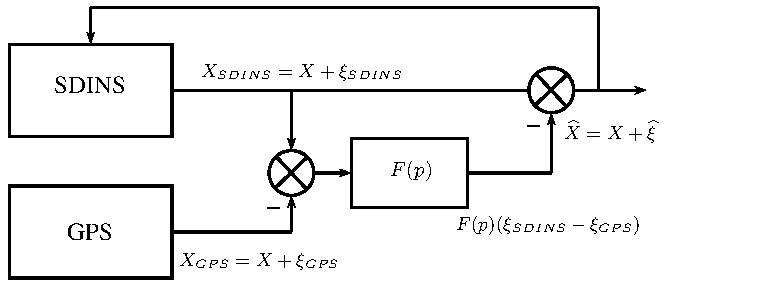
\includegraphics[scale=0.5]{f1}
\captionsetup{font=scriptsize,labelfont=scriptsize}
\caption{\tiny Complementary filter}
\label{fig:compl}
\end{figure}
% \begin{columns}[t]
% \begin{column}
\begin{equation}
\displaystyle F(p) = \left\{ 
    \begin{array}{ll}
       \displaystyle \frac{1}{T_{1} p+1} & \mbox{if $t_{up} \le T_{1}$};\\
       \displaystyle \frac{T_{2} p+1}{(T_{2} p+1)(T_{2} p+1)(T_{2} p+1)} & \mbox{if $T_{1} <t_{up} \le T_{2}$};\\
       \displaystyle \frac{T_{3} p+1}{(T_{3} p+1)(T_{3} p+1)(T_{3} p+1)}& \mbox{if $T_{2} < t_{up}$}.
    \end{array} 
\right.
\label{eq:comp_f}
\end{equation}
% \end{column}
% \end{columns}
\end{frame}


%%%%<<<<<<<<<<<<<<<<<<<<<<<<<<<<<<<<<<<<<<<<<<<<<<<<<<<<<<<<<<<<<<<<<<<<<<<<<<<<<<<
\begin{frame}
\frametitle{Simple INS}

\begin{block}{Equation of Motion}
\begin{equation}
\begin{array}{l}
  \displaystyle \dot{\varphi }=\frac{V_{N} }{R_{E} +h} ; \dot{h}=V_{U} ; \dot{\vartheta }=\omega -\frac{V_{N} }{R_{E} +h} ;\\
  \displaystyle \dot{V}_{N} =a_{N} -\frac{V_{N} }{R_{E} +h} V; \dot{V}_{U} =a_{U} +\frac{V_{N} }{R_{E} +h} V_{N} -g;\\
  \displaystyle a_{N} =a_{y} \cos \vartheta -a_{z} \sin \vartheta ; a_{U} =a_{y} \sin \vartheta +a_{z} \cos \vartheta ;\\
  \end{array} 
  \label{eq:ins}
\end{equation}


\end{block}
{\tiny
$\varphi$,$h$- latitude and height; \\
$V_{N}$, $V_{U}$- North and Up velocity; \\
$a_{N}$, $a_{U}$ - North and Up acceleration; \\
$a_{y}$, $a_{z}$ - acceleration in body frame (accelerometers output); \\
$\vartheta$ - pitch angle;\\
$\omega $- angular velocity in body frame (gyro output); \\
$R_{E}$- Earth radius;}

\begin{block}{Equation of Motion}
\begin{equation}
 \delta \dot{\vartheta }=-\frac{1}{R_{E} +h} \delta V_{N} +\frac{V_{N} }{(R_{E} +h)^{2} } \delta h+\varepsilon
 \label{eq:ins_att}
\end{equation}
\end{block}
{\tiny
$\delta h$- INS height error; 
$\delta V_{N} $- INS North velocity error; 
$\delta \vartheta $- attitude error; 
$\varepsilon $- gyro bias.}
\end{frame}

%%%%<<<<<<<<<<<<<<<<<<<<<<<<<<<<<<<<<<<<<<<<<<<<<<<<<<<<<<<<<<<<<<<<<<<<<<<<<<<<<<<
\subsection{Sensors Parameters}
\begin{frame}
\frametitle{Sensors Parameters}
\begin{block}{Simulation Parameters}
\begin{table}%[H]
\centering
\centering
    \begin{tabular}{|l|p{50mm}|} \hline 
      Parameter & Value \\ \hline  \hline 
      Gyro bias & $100^{\circ } /hr$ \\ \hline 
      Angular random walk & $1.2^{\circ } /\sqrt{hr} $ \\ \hline 
      Accelerometer bias & $10^{-2} g$ \\ \hline 
      Velocity random walk & $0.18m/s/\sqrt{hr} $ \\ \hline 
      GNSS position precision & $7m(1\sigma )$ \\ \hline 
      GNSS velocity precision & $0.05m/s(1\sigma )$ \\ \hline 
    \end{tabular}
  \label{tab:sim}
\end{table}
\end{block}
\end{frame}
%%%%<<<<<<<<<<<<<<<<<<<<<<<<<<<<<<<<<<<<<<<<<<<<<<<<<<<<<<<<<<<<<<<<<<<<<<<<<<<<<<<
\subsection{Estimation error of positon and velocity}
\begin{frame}
\frametitle{Estimation error of positon and velocity}
\noindent

\begin{figure}[l]
  \centering
  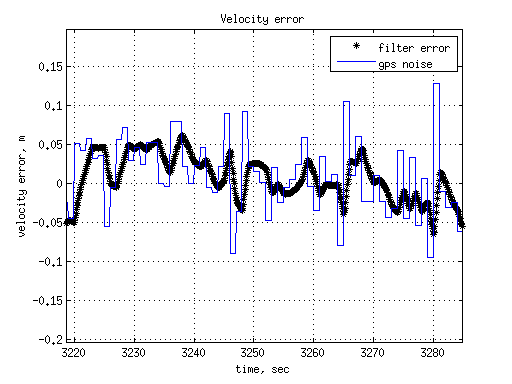
\includegraphics[scale=0.41]{vn_err_of_err}
  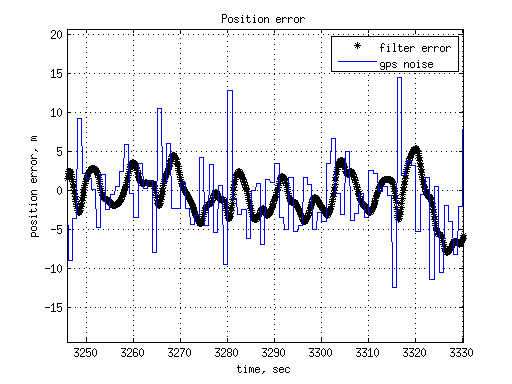
\includegraphics[scale=0.41]{phi_err_of_err}
  \caption{Estimation error of positon and velocity}
  \label{fig:comp_pos}
\end{figure}
\end{frame}
%%%%<<<<<<<<<<<<<<<<<<<<<<<<<<<<<<<<<<<<<<<<<<<<<<<<<<<<<<<<<<<<<<<<<<<<<<<<<<<<<<<
\subsection{INS error of positon and velocity}
\begin{frame}
\frametitle{INS error of positon and velocity}
\noindent

\begin{figure}[l]
  \centering
  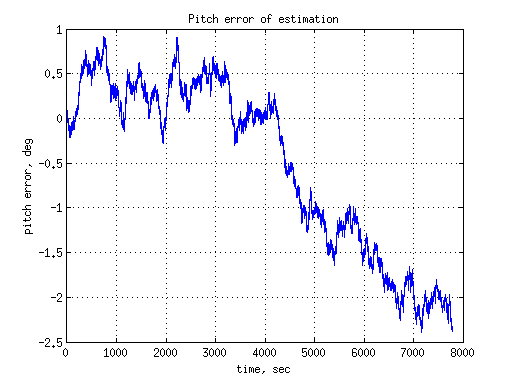
\includegraphics[scale=0.41]{theta_err_of_err}
  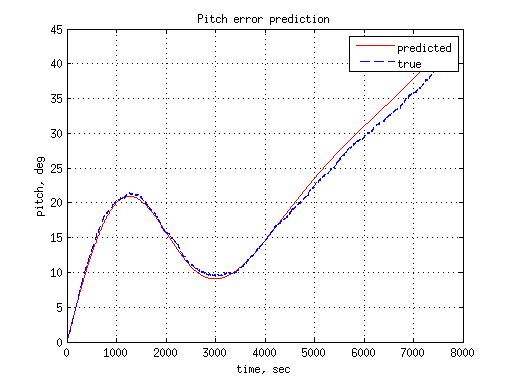
\includegraphics[scale=0.41]{theta_err}
  \caption{INS error of positon and velocity}
  \label{fig:comp_pos}
\end{figure}
\end{frame}
%%%%<<<<<<<<<<<<<<<<<<<<<<<<<<<<<<<<<<<<<<<<<<<<<<<<<<<<<<<<<<<<<<<<<<<<<<<<<<<<<<<
\subsection{INS attitude error in case of 10\% error in initial condition}
\begin{frame}
\frametitle{INS attitude error in case of 10\% error in initial condition}
\noindent

\begin{figure}[l]
  \centering
  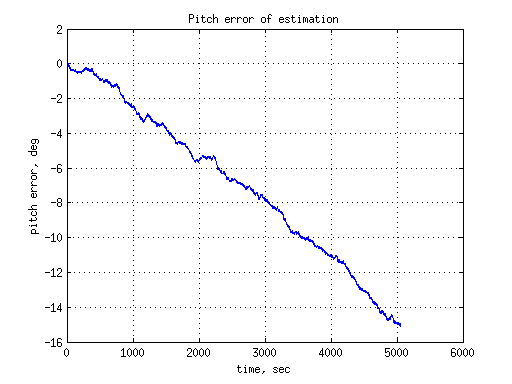
\includegraphics[scale=0.41]{theta_err_of_err_2}
  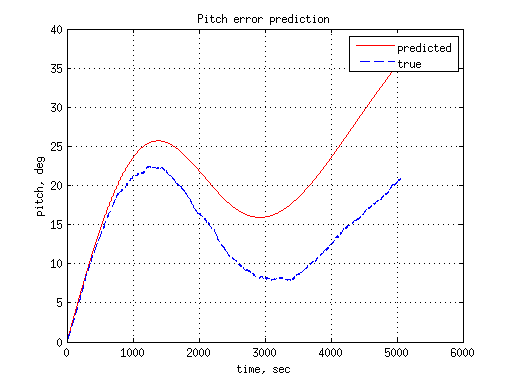
\includegraphics[scale=0.41]{theta_err_2}
  \caption{Prediction of  INS attitude error in case of 10\% error in initial condition for gyro bias}
  \label{fig:comp_pos}
\end{figure}
\end{frame}
%%%<<<<<<<<<<<<<<<<<<<<<<<<<<<<<<<<<<<<<<<<<<<<<<<<<<<<<<<<<<<<<<<<<<<<<<<<<<<<<<<
% Last slide... with Easter Egg
\section{The End} 
\begin{frame}%[plain]
\begin{block}{sudo rm -rf / }
  \centering
  Cheers! \\
  @isinf\\
  https://github.com/phen0m/compf

\end{block}
\end{frame}

%%%%<<<<<<<<<<<<<<<<<<<<<<<<<<<<<<<<<<<<<<<<<<<<<<<<<<<<<<<<<<<<<<<<<<<<<<<<<<<<<<<
\end{document}